\documentclass{../source/Experiment}

\major{信息工程}
\name{姚桂涛}
\title{喇叭天线的幅射特性测量及CST仿真}
\stuid{3190105597}
\college{信息与电子工程学院}
\date{\today}
\lab{东4-221}
\course{电磁场与电磁波}
\instructor{王子立}
\grades{}
\expname{喇叭天线的幅射特性测量及CST仿真}
\exptype{}
\partner{}

\usepackage{caption}

\DeclareCaptionLabelSeparator{twospace}{\, }
\captionsetup{labelsep = twospace}

\begin{document}
    \makecover
    \makeheader

    \begin{center}
        \bfseries\Large{矩形波导馈电的角锥喇叭天线CST仿真}
    \end{center}
    \section{实验目的}
        \begin{enumerate}
            \item 了解并掌握波导喇叭天线的常用参数指标和分析方法.
            \item 了解熟悉CST软件的基本使用方法,学会运用其进行建模、仿真。
        \end{enumerate}
    \section{实验任务}
        用CST软件对特定的巨型波导喇叭天线进行建模、仿真,分析其辐射特性,并与喇叭天线辐射特性测量实验进行比较。
    \section{实验过程与结果}
        \subsection{模型建立}
            \subsubsection{建立工程}
                \begin{figure}[H]
                    \centering
                    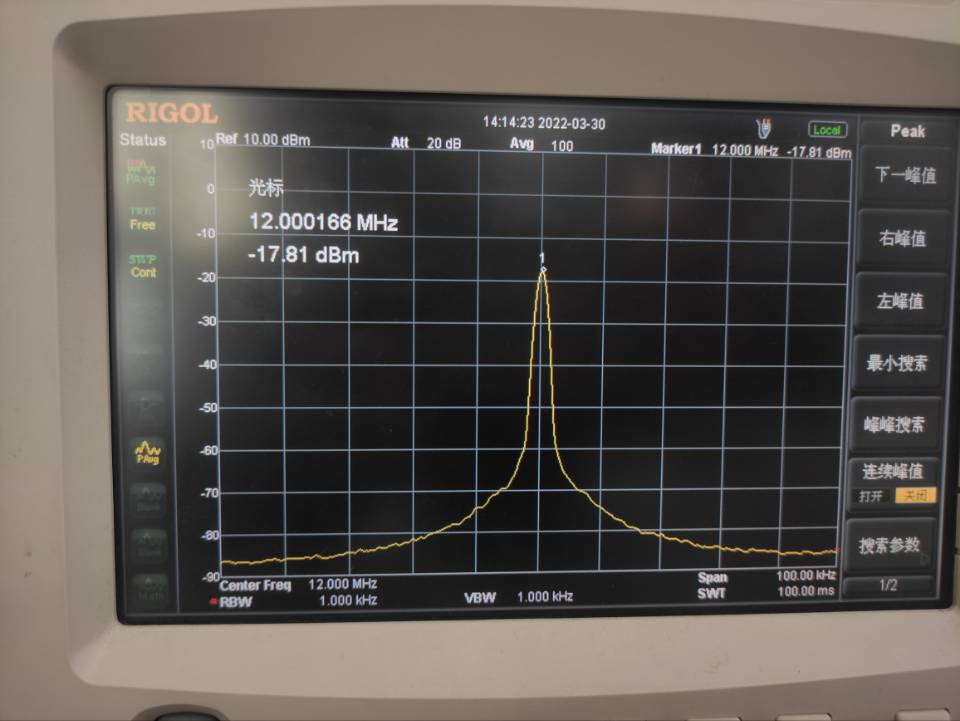
\includegraphics[width = 0.6\textwidth]{1}
                    \caption{}
                \end{figure}

                \begin{figure}[H]
                    \centering
                    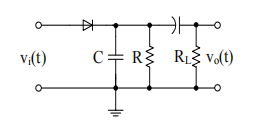
\includegraphics[width = 0.6\textwidth]{2}
                    \caption{}
                \end{figure}


            \subsubsection{参数设置}
                \begin{figure}[H]
                    \centering
                    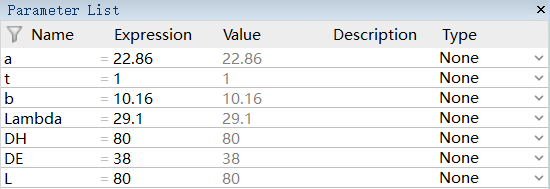
\includegraphics[width = 0.6\textwidth]{0}
                    \caption{}
                \end{figure}
            \subsubsection{创建矩形}

            \begin{figure}[H]
                \centering
                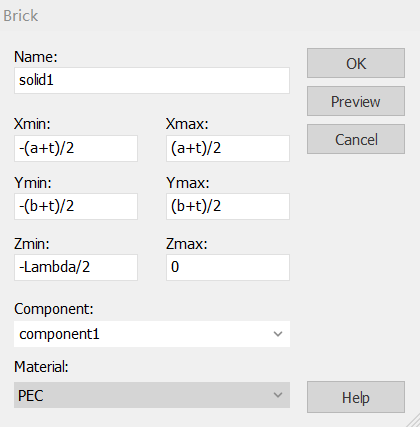
\includegraphics[width = 0.5\textwidth]{3}
                \caption{}
            \end{figure}
            
            \begin{figure}[H]
                \centering
                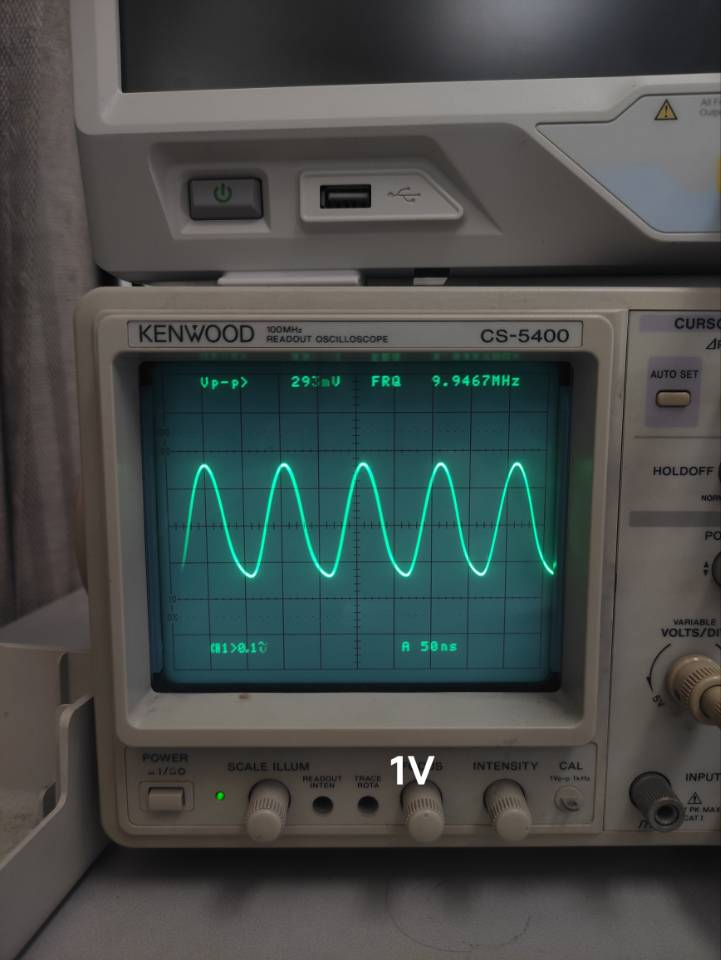
\includegraphics[width = 0.8\textwidth]{4}
                \caption{}
            \end{figure}
            
            \subsubsection{建立喇叭模型}

            建立喇叭口径面
            \begin{figure}[H]
                \centering
                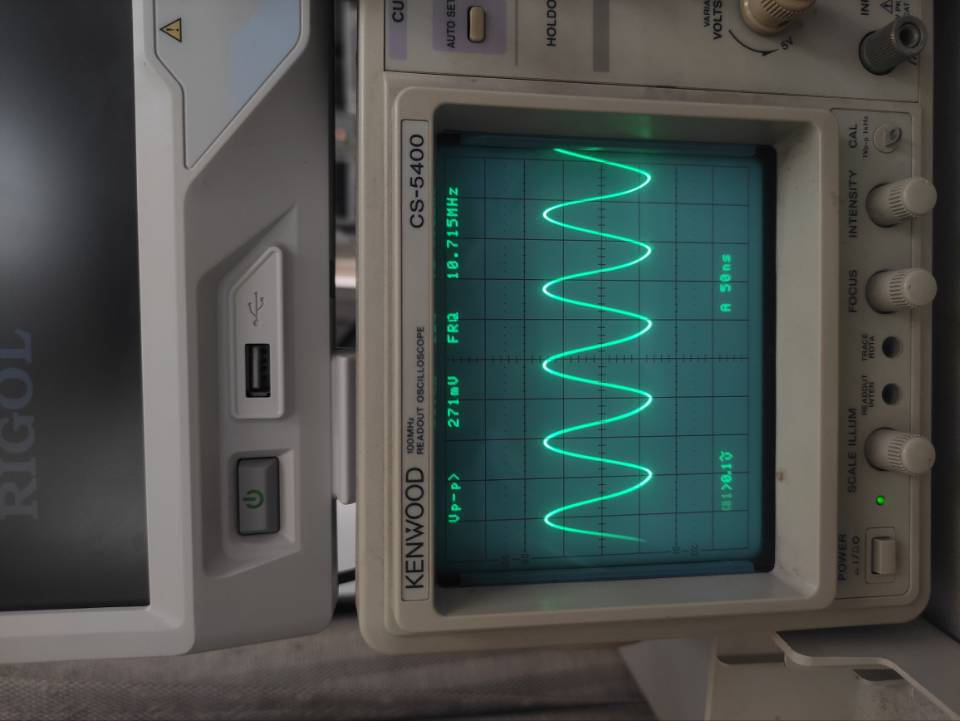
\includegraphics[width = 0.4\textwidth]{5}
                \caption{}
            \end{figure}

            \begin{figure}[H]
                \centering
                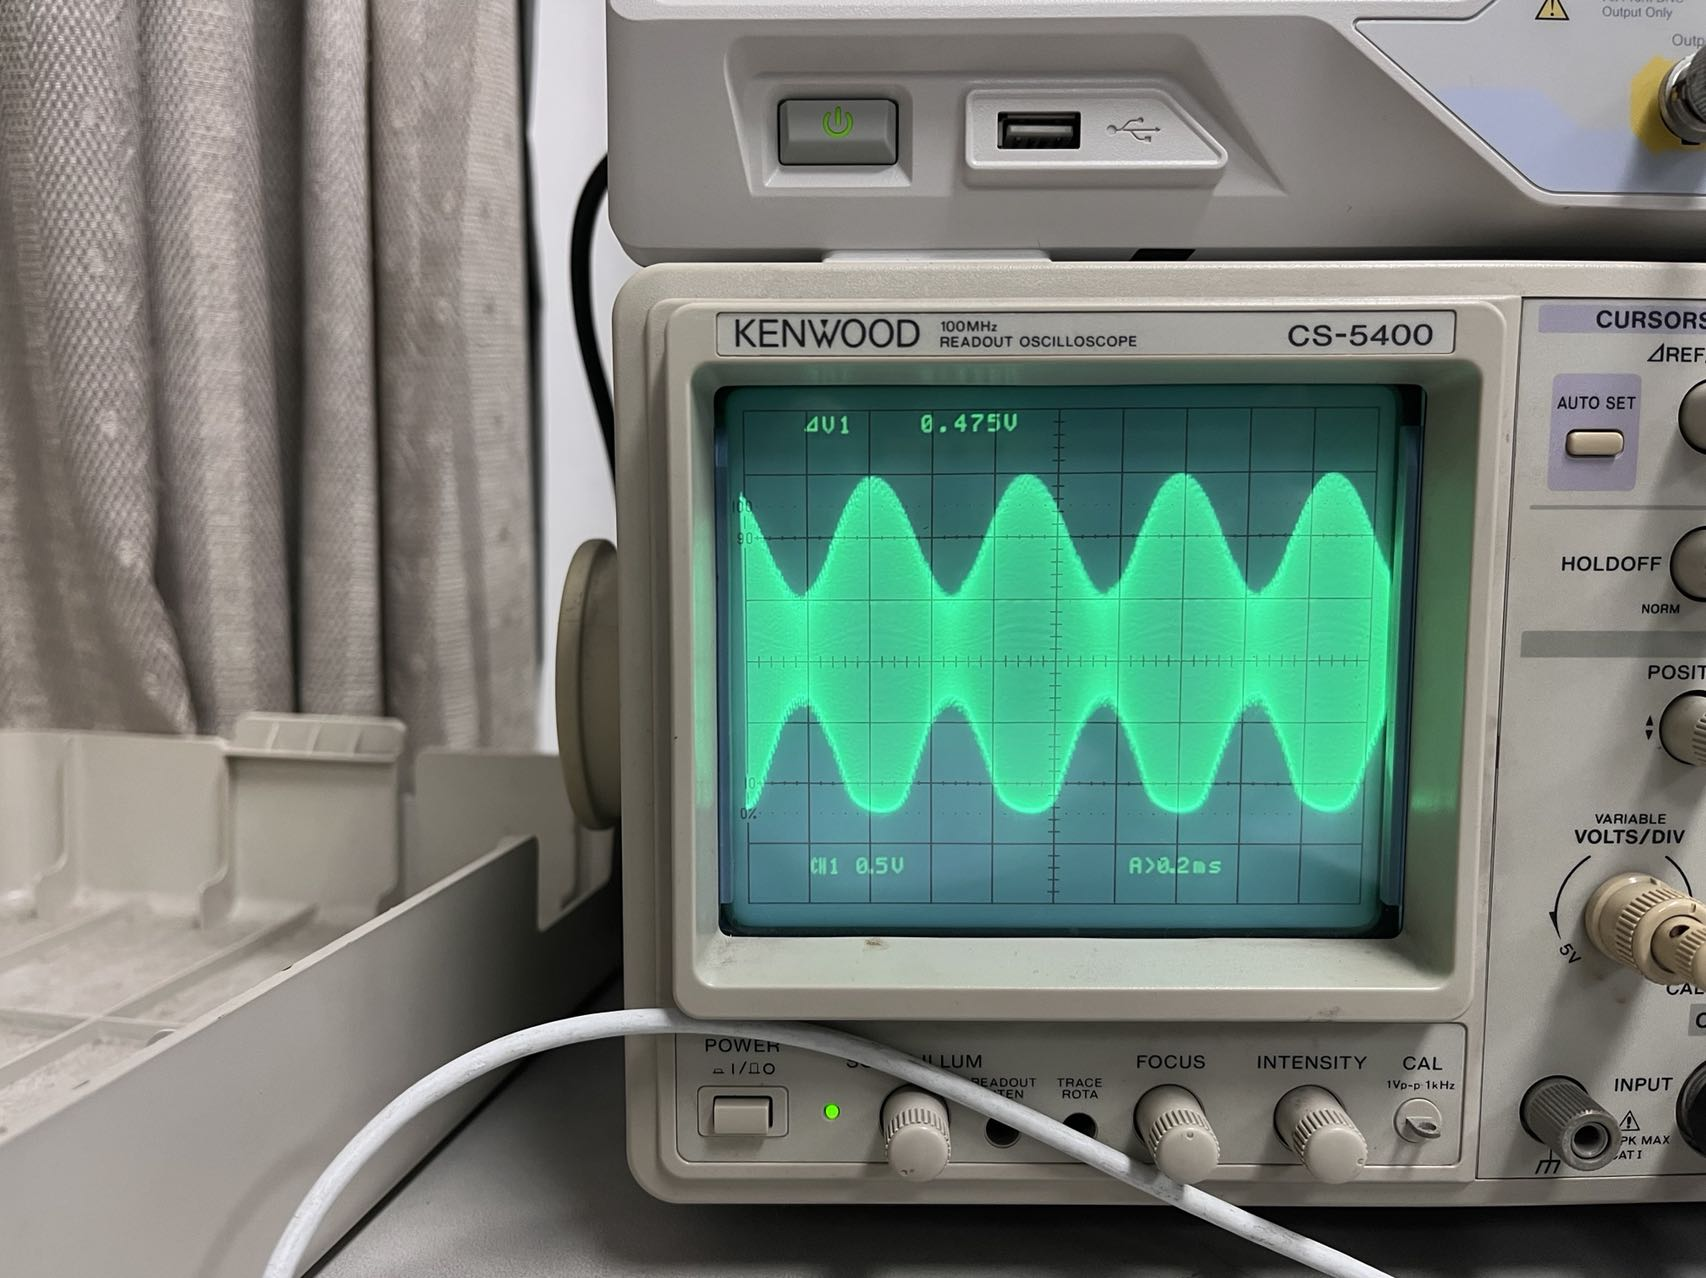
\includegraphics[width = 0.4\textwidth]{7}
                \caption{}
            \end{figure}

            \begin{figure}[H]
                \centering
                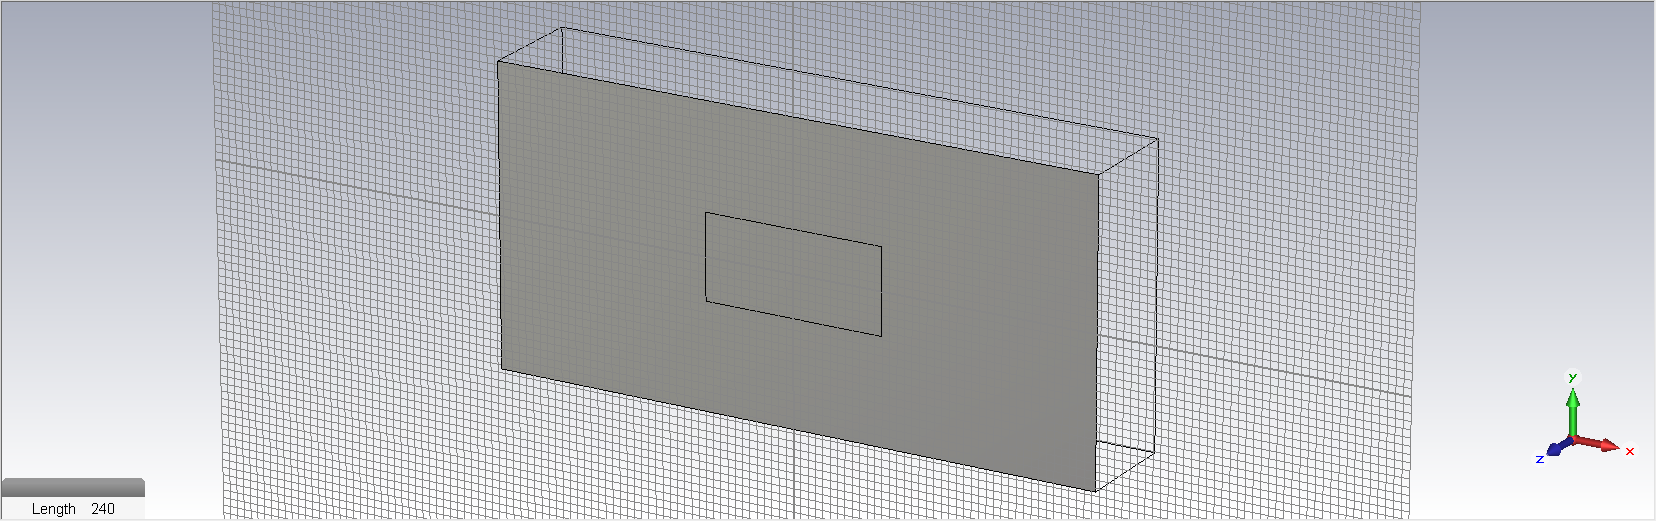
\includegraphics[width = 0.8\textwidth]{8}
                \caption{}
            \end{figure}


            设置喇叭口径面的空间位置

            \begin{figure}[H]
                \centering
                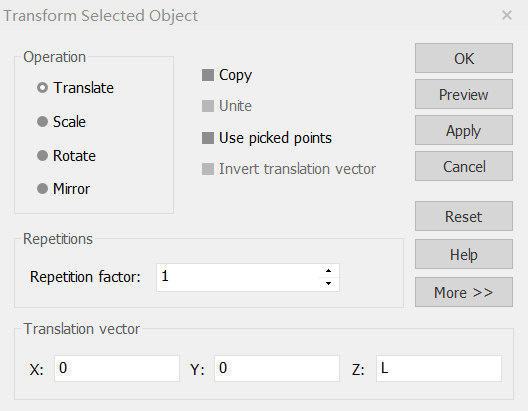
\includegraphics[width = 0.6\textwidth]{9}
                \caption{}
            \end{figure}


            \begin{figure}[H]
                \centering
                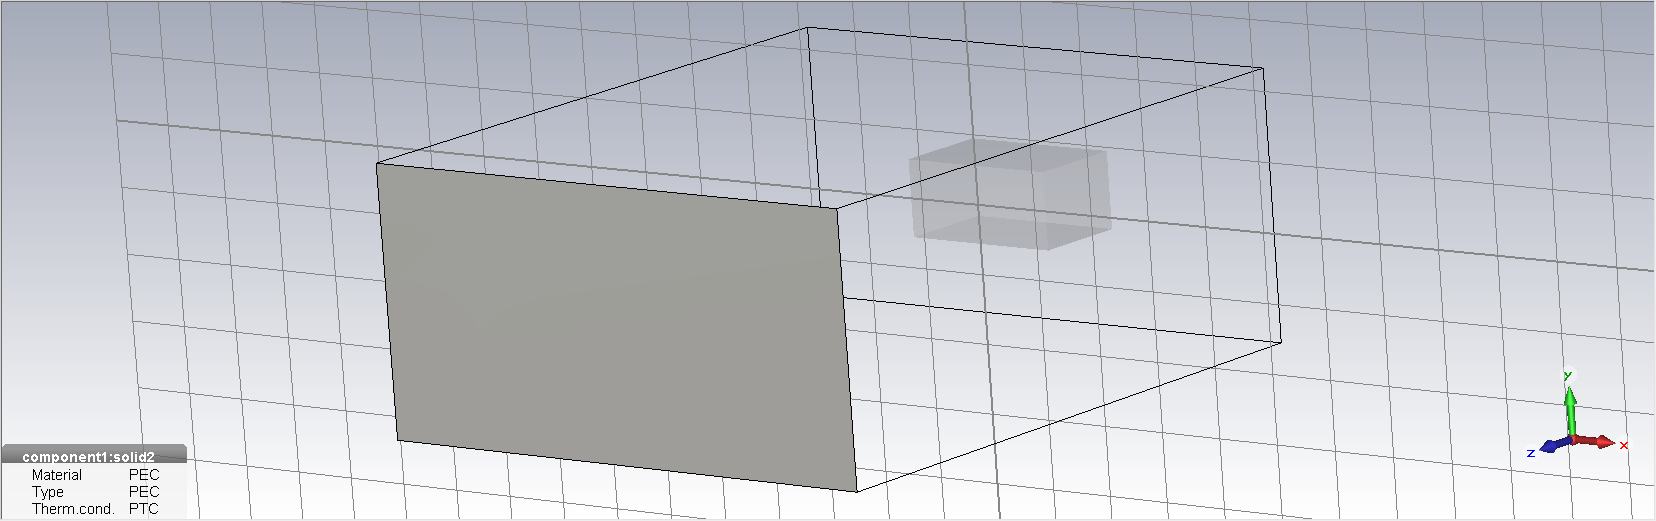
\includegraphics[width = 0.8\textwidth]{10}
                \caption{}
            \end{figure}
            创建喇叭侧壁
            \begin{figure}[H]
                \centering
                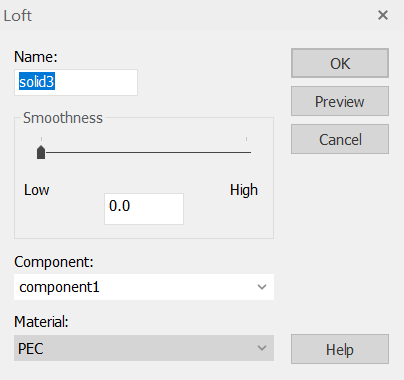
\includegraphics[width = 0.4\textwidth]{11}
                \caption{}
            \end{figure}
            \begin{figure}[H]
                \centering
                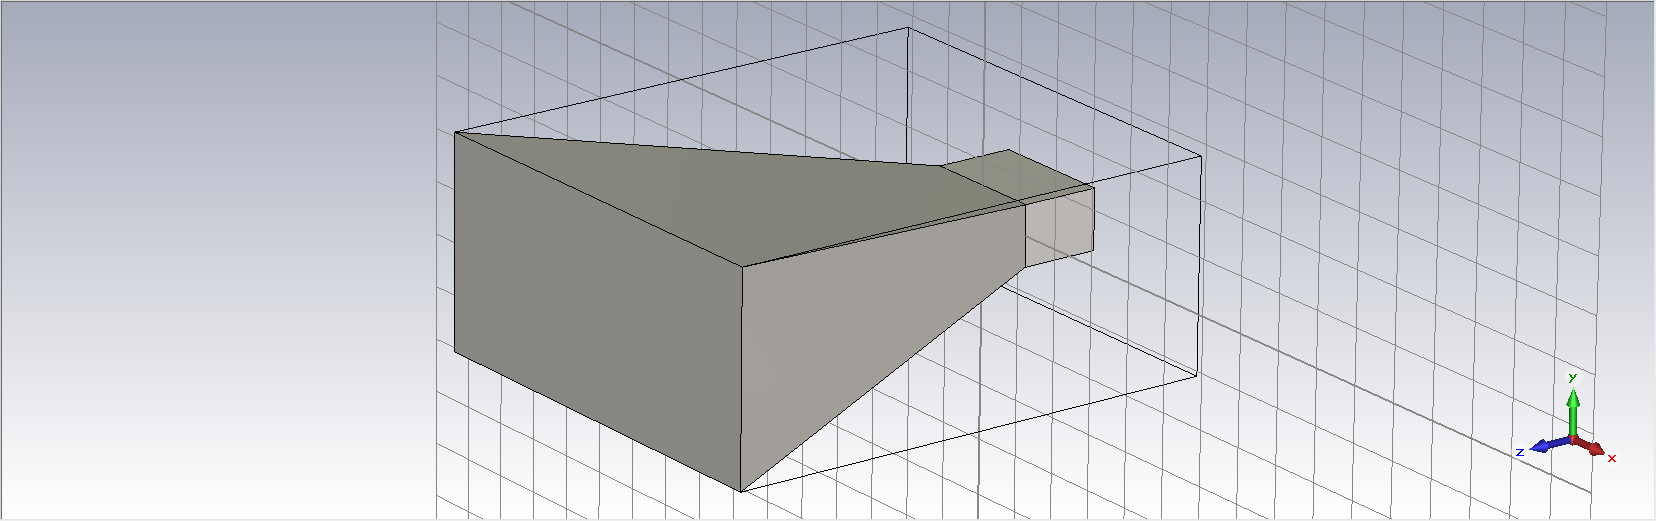
\includegraphics[width = 0.8\textwidth]{12}
                \caption{}
            \end{figure}

            掏空
            \begin{figure}[H]
                \centering
                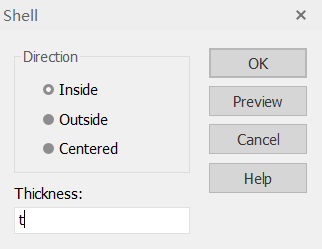
\includegraphics[width = 0.4\textwidth]{13}
                \caption{}
            \end{figure}
            \begin{figure}[H]
                \centering
                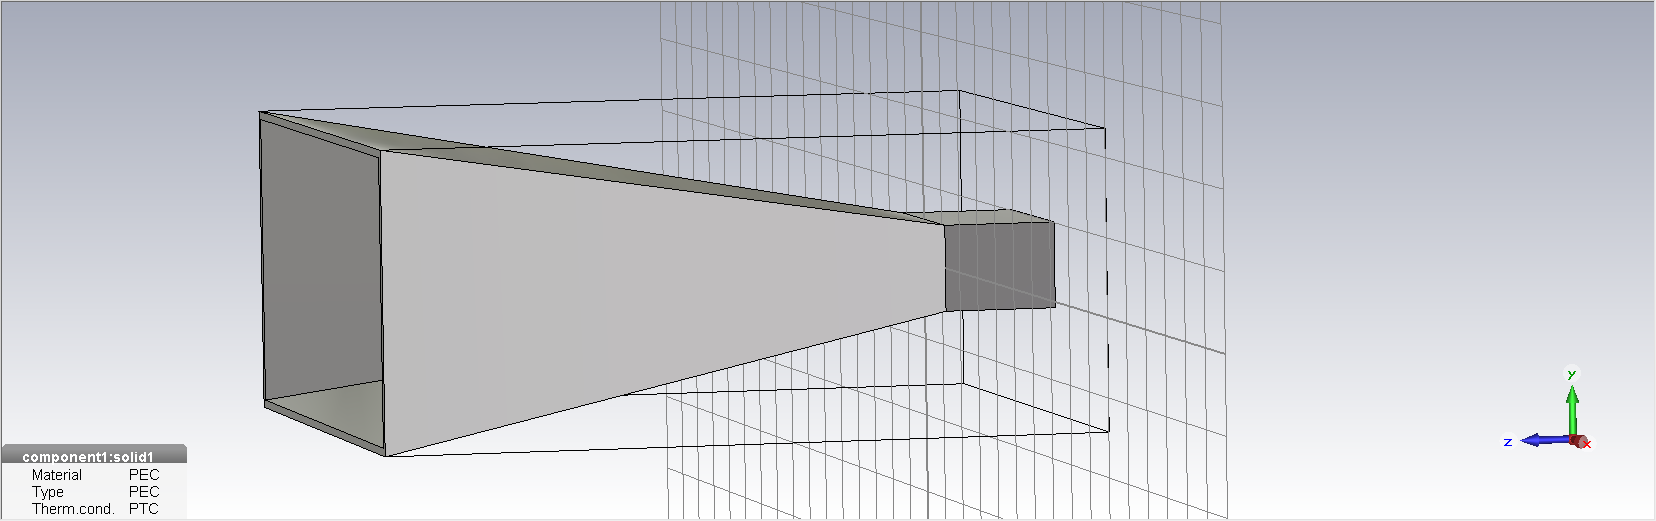
\includegraphics[width = 0.8\textwidth]{14}
                \caption{}
            \end{figure}

        \subsection{仿真分析}

            \subsubsection{仿真条件设置}
            仿真频率
            \begin{figure}[H]
                \centering
                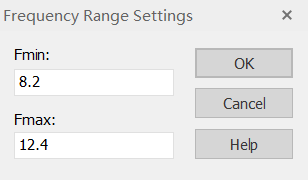
\includegraphics[width = 0.3\textwidth]{15}
                \caption{}
            \end{figure}
            仿真边界条件
            \begin{figure}[H]
                \centering
                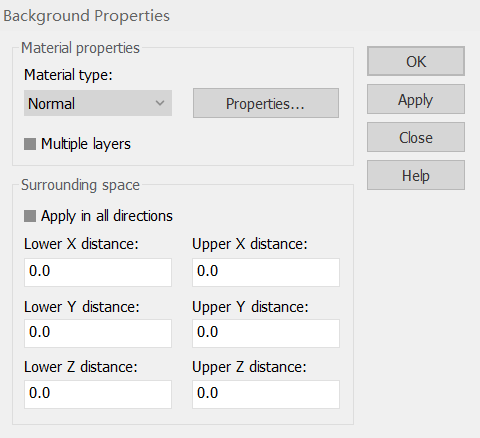
\includegraphics[width = 0.6\textwidth]{16}
                \caption{}
            \end{figure}
            
            \begin{figure}[H]
                \centering
                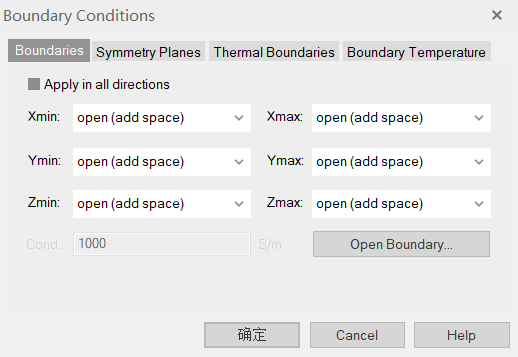
\includegraphics[width = 0.6\textwidth]{17}
                \caption{}
            \end{figure}

            端口设置
            \begin{figure}[H]
                \centering
                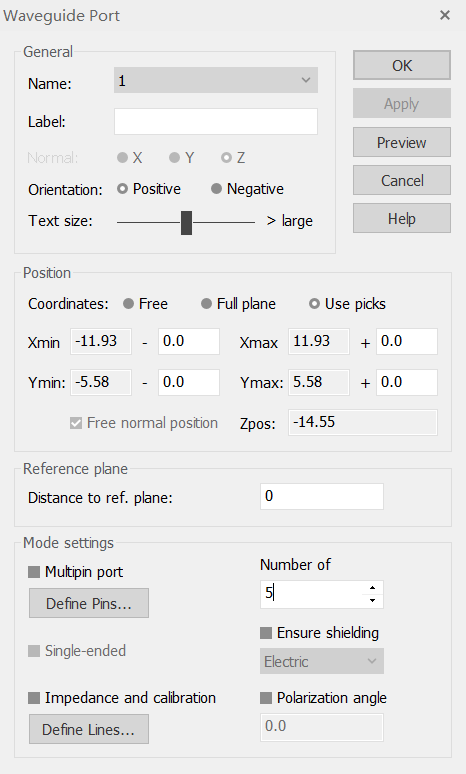
\includegraphics[width = 0.6\textwidth]{18}
                \caption{}
            \end{figure}
            设置监视器
            
            \begin{figure}[H]
                \centering
                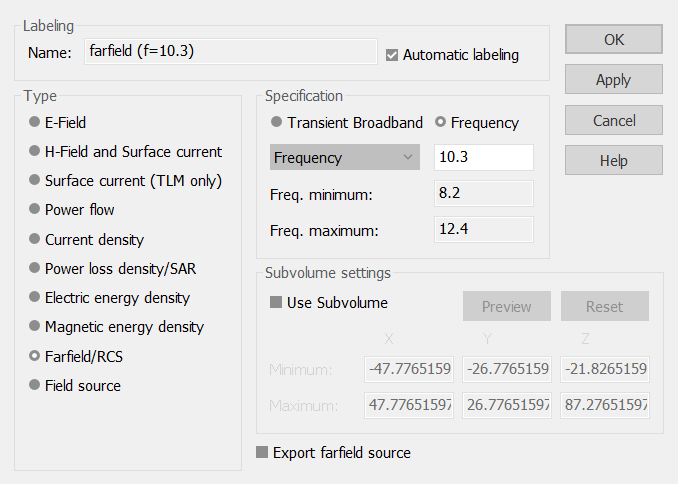
\includegraphics[width = 0.7\textwidth]{20}
                \caption{}
            \end{figure}
            \begin{figure}[H]
                \centering
                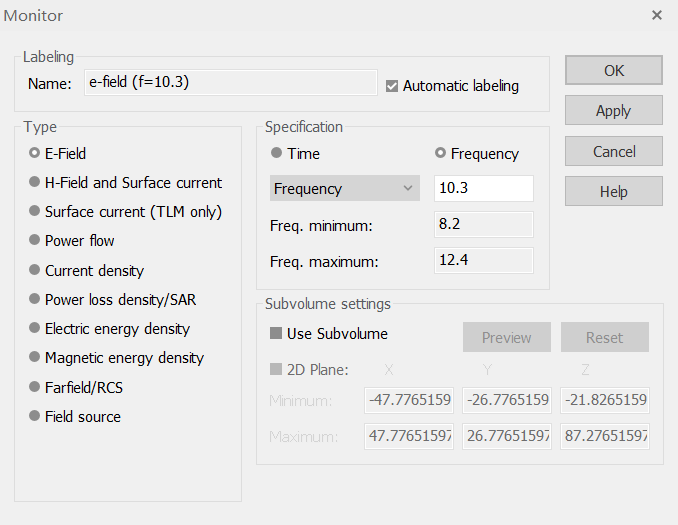
\includegraphics[width = 0.7\textwidth]{24}
                \caption{}
            \end{figure}
            \begin{figure}[H]
                \centering
                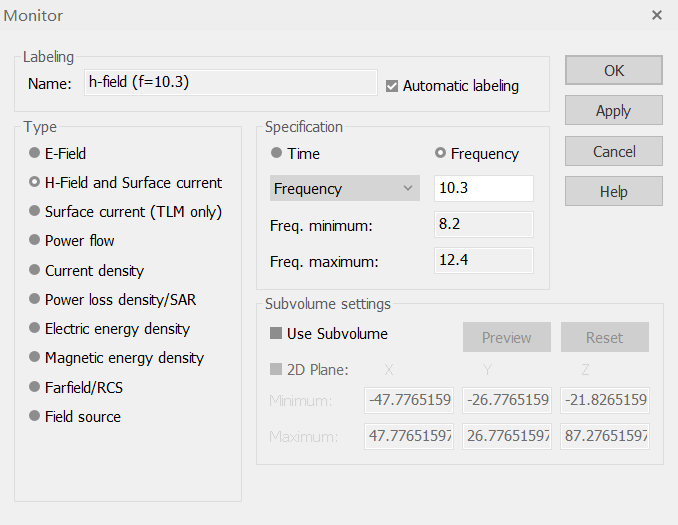
\includegraphics[width = 0.7\textwidth]{25}
                \caption{}
            \end{figure}
            
            \subsubsection{模式分析}
            \begin{figure}[H]
                \centering
                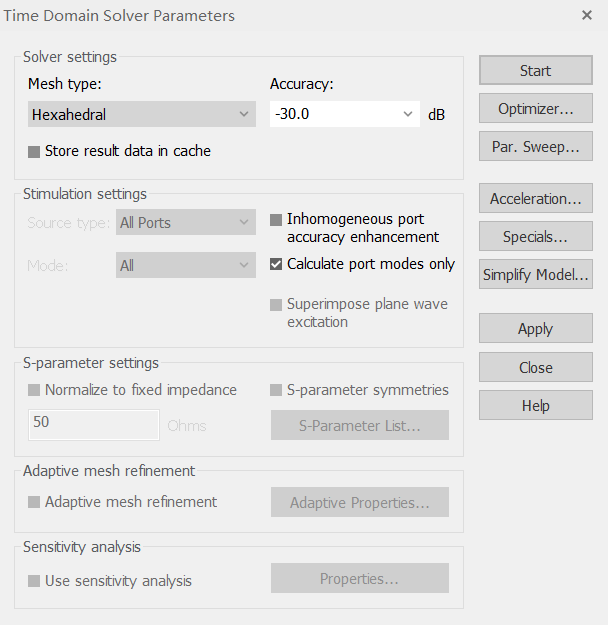
\includegraphics[width = 0.7\textwidth]{21}
                \caption{}
            \end{figure}
            \begin{figure}[H]
                \centering
                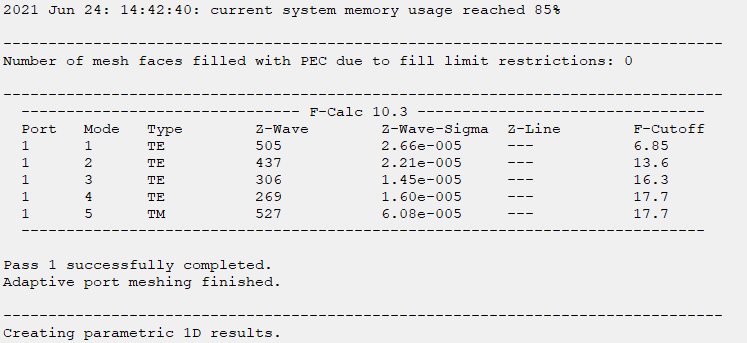
\includegraphics[width = 0.7\textwidth]{22}
                \caption{}
            \end{figure}
            

            由于仿真最高频率为12.4GHz,所以在这种结构的喇叭天线中只传输1 种模式的波,设置的吸收的模式数只要大于1 就可以了。
            \subsubsection{仿真设置}
            \begin{figure}[H]
                \centering
                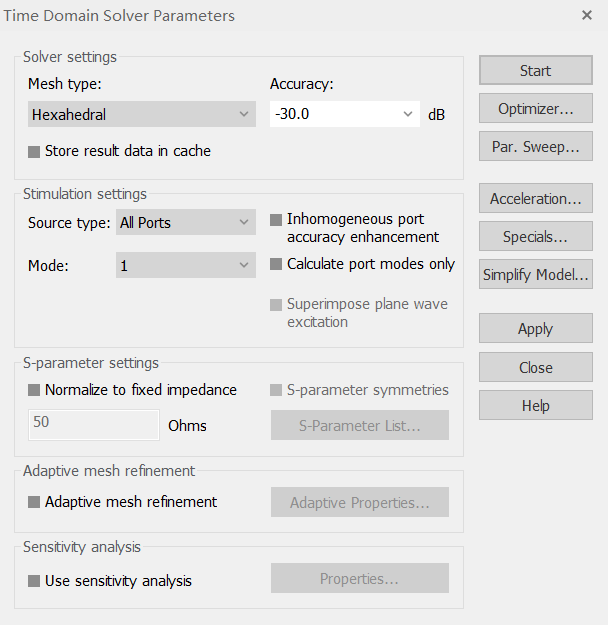
\includegraphics[width = 0.7\textwidth]{23}
                \caption{}
            \end{figure}
            
        \subsection{仿真结果}

            \subsubsection{$S_{11}$曲线}
            \begin{figure}[H]
                \centering
                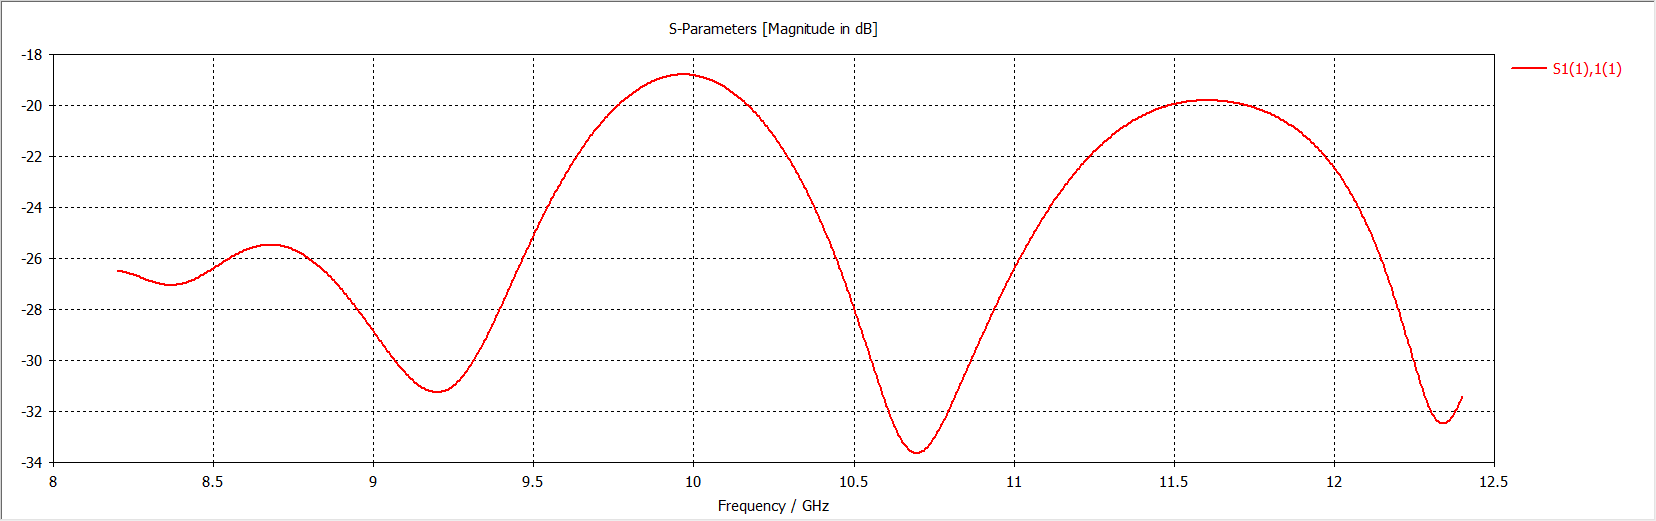
\includegraphics[width = 0.8\textwidth]{S11}
                \caption{}
            \end{figure}
            
            \subsubsection{驻波曲线}
            \begin{figure}[H]
                \centering
                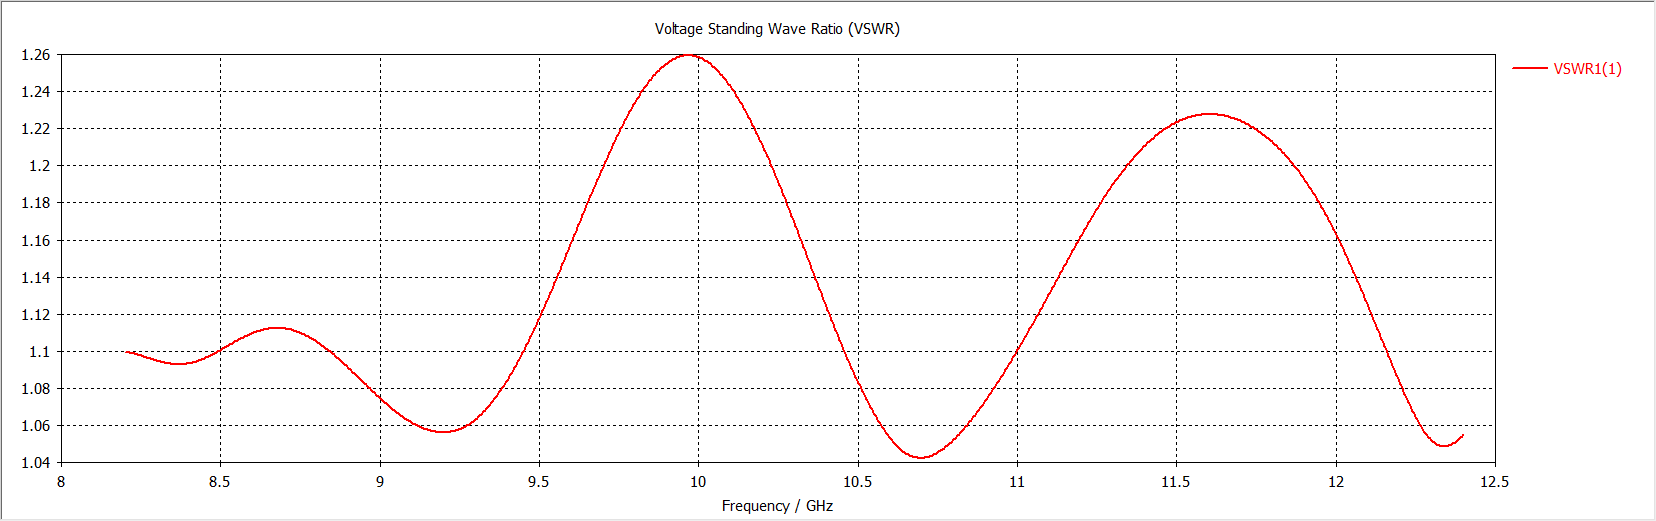
\includegraphics[width = 0.8\textwidth]{VSWR}
                \caption{}
            \end{figure}
            
            \subsubsection{方向图}
            \begin{figure}[H]
                \centering
                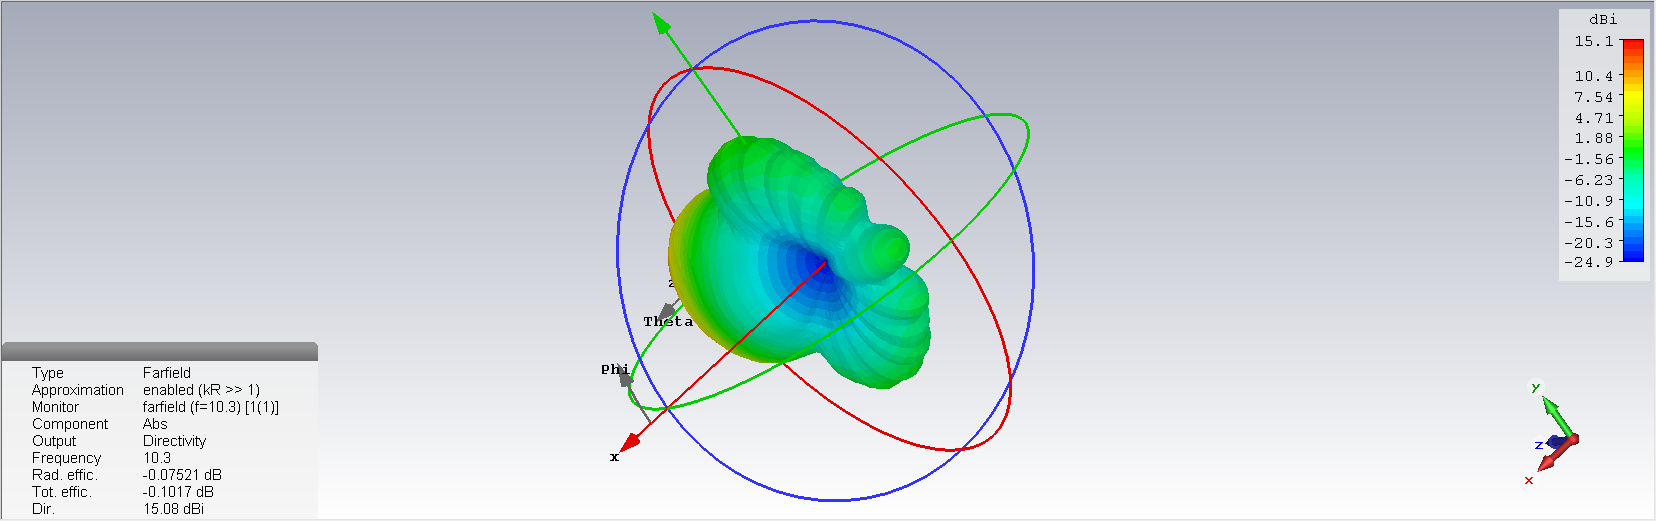
\includegraphics[width = 0.8\textwidth]{Directivity}
                \caption{}
            \end{figure}
            \begin{figure}[H]
                \centering
                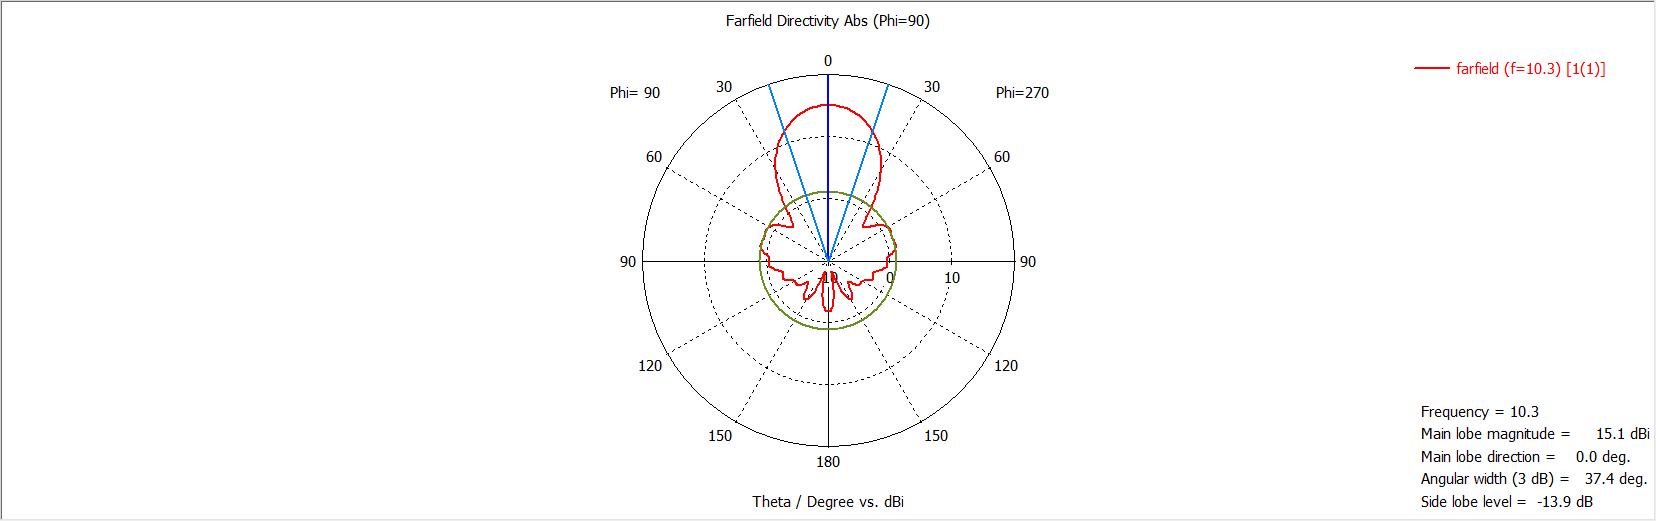
\includegraphics[width = 0.8\textwidth]{Directivity Polar}
                \caption{}
            \end{figure}
            
            \subsubsection{增益图}
            \begin{figure}[H]
                \centering
                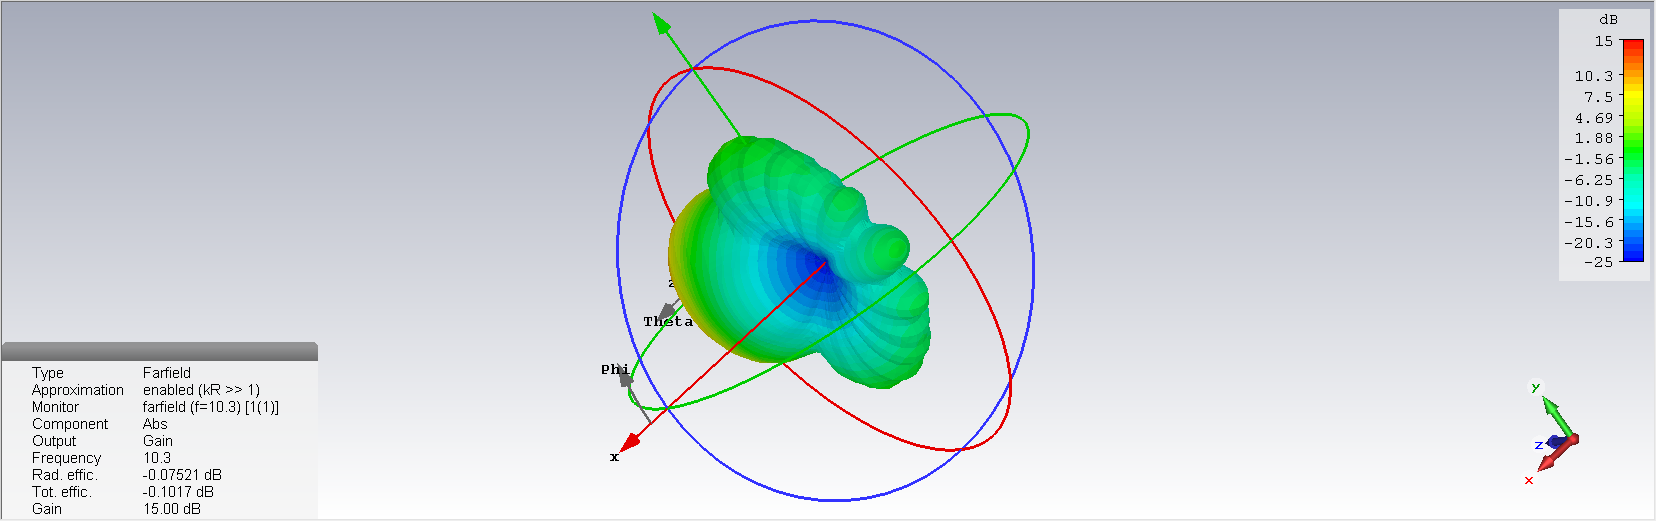
\includegraphics[width = 0.8\textwidth]{Gain}
                \caption{}
            \end{figure}
            \begin{figure}[H]
                \centering
                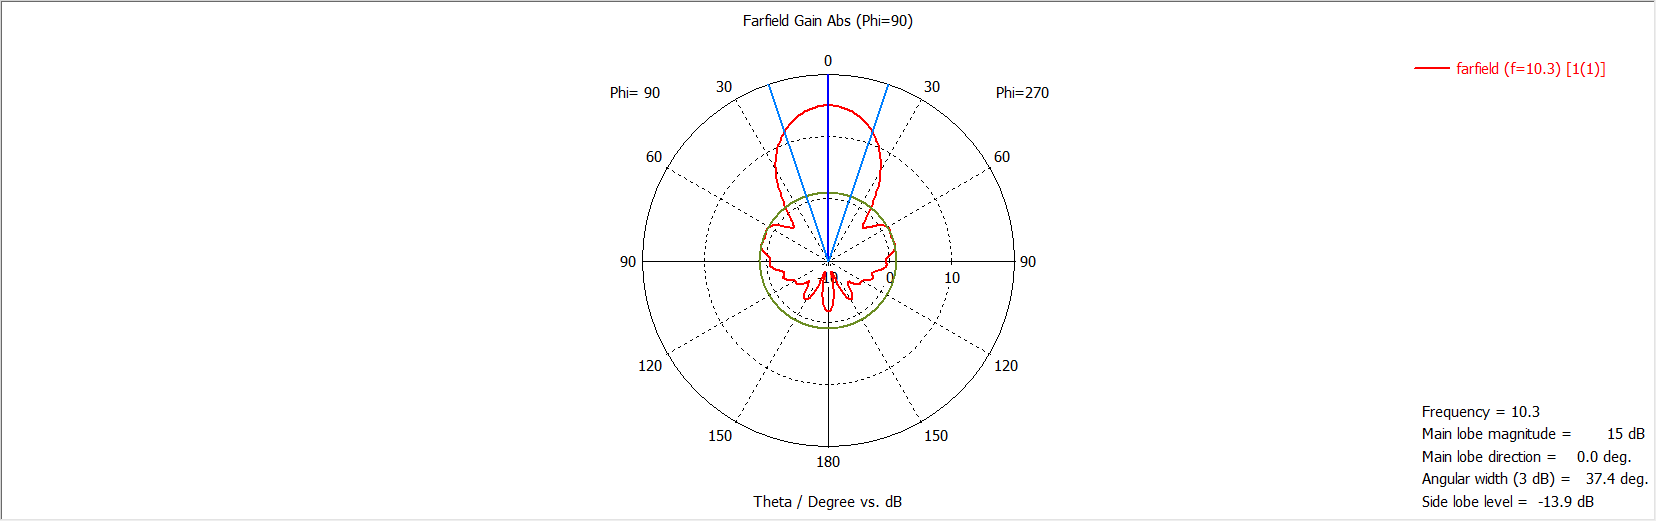
\includegraphics[width = 0.8\textwidth]{Gain polar}
                \caption{}
            \end{figure}
            
            \subsubsection{E-field,  H-field,  surface current图}
            \begin{figure}[H]
                \centering
                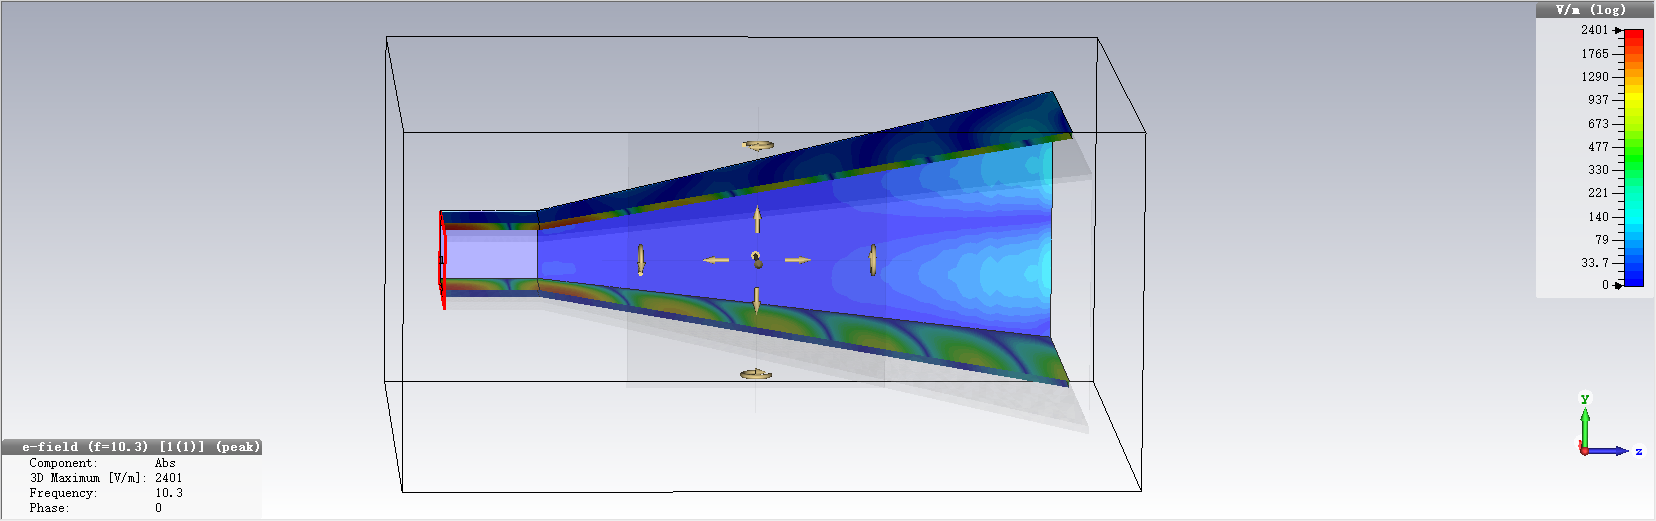
\includegraphics[width = 0.8\textwidth]{e-field}
                \caption{e-field}
            \end{figure}
            \begin{figure}[H]
                \centering
                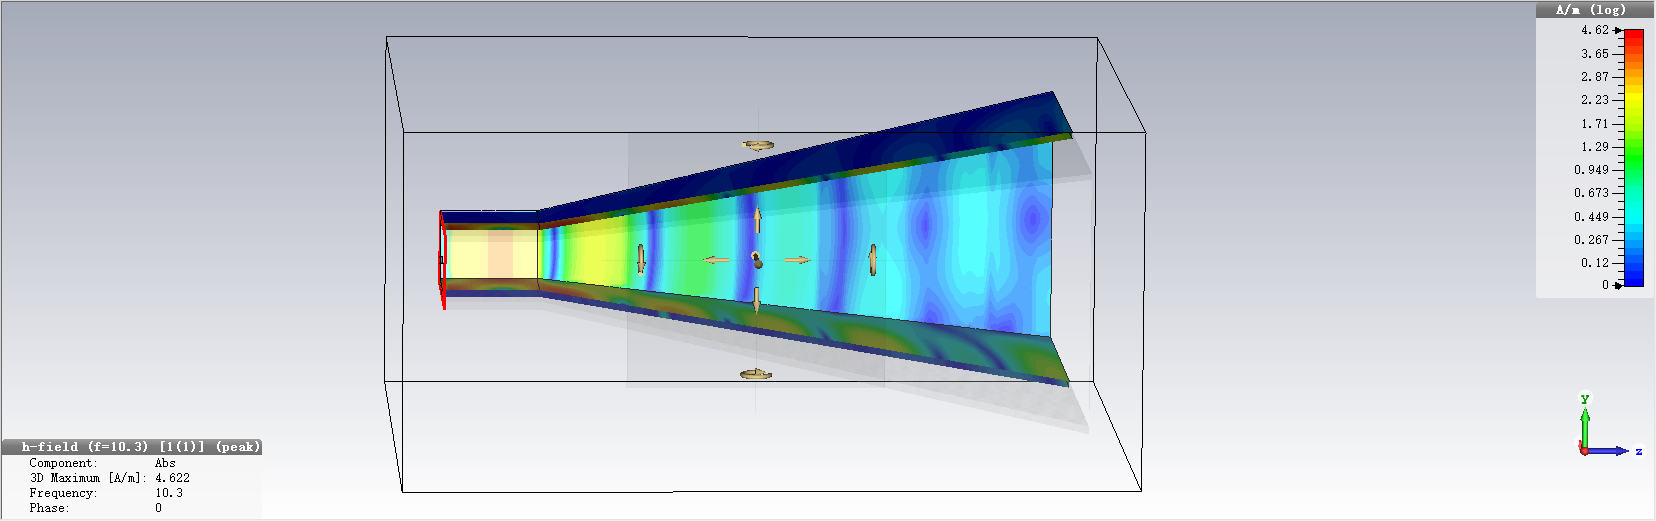
\includegraphics[width = 0.8\textwidth]{h-field}
                \caption{h-field}
            \end{figure}
            \begin{figure}[H]
                \centering
                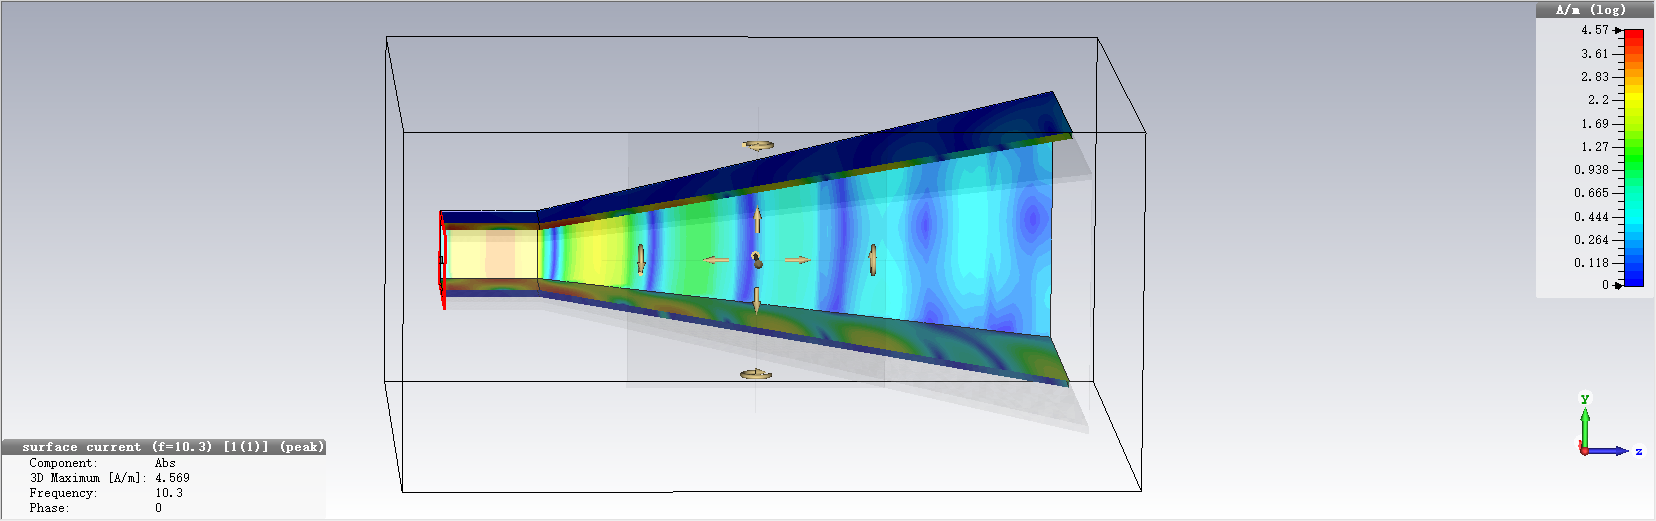
\includegraphics[width = 0.8\textwidth]{surface}
                \caption{surface current}
            \end{figure}
            
        \subsection{分析结论}

            从仿真结果来看,该矩形波导馈电的角锥喇叭天线的主瓣方向为$ \varphi = 0 \deg ,\, \theta = 0 \deg$,主瓣宽度为37.4\degree ,主瓣的最大增益为15dB,最大增益的仿真值与
            理论估计值相近。同时,该天线输入端口的反射系数在工作频段内均在20dB 以下,能够较好的工作。

    \section{实验收获与体会}

        
    \setcounter{section}{0}
\end{document}